\documentclass{beamer}
%
% Choose how your presentation looks.
%
% For more themes, color themes and font themes, see:
% http://deic.uab.es/~iblanes/beamer_gallery/index_by_theme.html
%
% to be used by pdfpc: https://pdfpc.github.io/
% guide at https://github.com/pdfpc/pdfpc/releases/latest/download/pdfpc-demo.pdf
%
% command to use for this presentation:
% pdfpc --size=1920:1060 DEC_federated_EN.pdf
\mode<presentation>
{
  \usetheme{Darmstadt} % or try Darmstadt, Madrid, Warsaw, ... (default)
  \usecolortheme{crane} % or try albatross, beaver, crane, ... (deafult)
  \usefonttheme{structurebold}  % or try serif, structurebold, ... (deafult)
  \setbeamertemplate{navigation symbols}{}
  \setbeamertemplate{caption}[numbered]
  \setbeameroption{show notes} %un-comment to see the notes
} 

\usepackage[english]{babel}
\usepackage[utf8x]{inputenc}
\usepackage{wrapfig}
\usepackage{multimedia}
\usepackage{multirow}
\usepackage{array}

\title[Unsupervised Clustering in Federated Learning]{DEC used in a federated setting}
\author{Lorenzo Sani}
\institute{Università degli Studi di Bologna}
\date{\today}

\begin{document}

\begin{frame}
  \titlepage
\end{frame}


\section{DEC}

\begin{frame}{Deep Embedding for Clustering (DEC)\cite{DBLP:journals/corr/XieGF15}}
	\begin{itemize}
	\item Aims:
		\begin{itemize}
			\item Learning feature representations of data\\($\mathbb{B}^{40}$ data space $\Rightarrow$ 	$\mathbb{R}^f$ feature space)
			\item Learning cluster assignments\\(number of clusters $f$ is an hyperparameter)
		\end{itemize}
	\end{itemize}
	\centering
	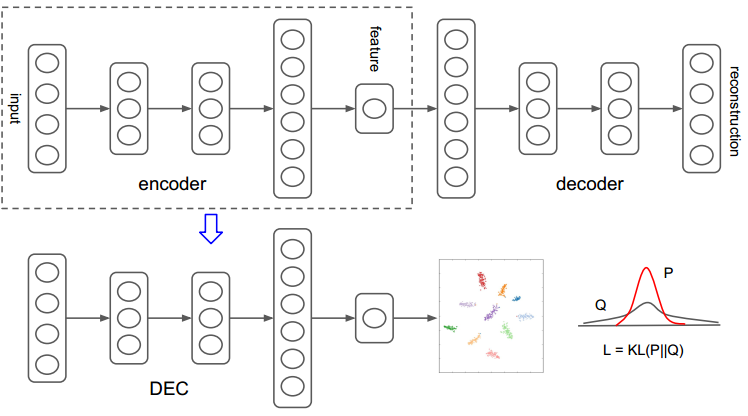
\includegraphics[width=0.58\textwidth, keepaspectratio]{./images/DEC_model.png}
	\begin{itemize}
		\item Stacked denoising Autoencoder (SAE)
		\item DNN optimized for the clustering objective
	\end{itemize}
\end{frame}

\begin{frame}{Stacked Denoising Autoencoder (SAE)}
	\begin{itemize}
		\item Random Flipping Noise for binary data, respecting the frequencies of the whole dataset
		\item 5 layer depth Dense Neural Network with random dropout, shapes: 40-26-26-100-$f$
		\item Tied Dense layers is used for the decoder part
		\item Constraints and regularizers typical for SAE were tested
		\begin{itemize}
			\item Unit Norm: constrains the weights incident to each hidden unit to have unit norm 
		\end{itemize}
		\item Binary Cross Entropy (BCE) loss function for reconstruction of binary data
	\end{itemize}
\end{frame}

\begin{frame}{Training of SAE}
	\begin{itemize}
		\item Pretrain
		\begin{itemize}
			\item 2500, or 5000 epochs
			\item dropout rate was set equal to random flipping rate,\\
				many values were tested, 20\%, 10\%, 5\%, 1\% 
			\item minimizing BCE optimized by Stochastic Gradient Descent,\\
				decaying learning rate, 0.1 then divided by 10 every 1000, or 2000 epochs
		\end{itemize}
		\item Finetune
		\begin{itemize}
			\item 5000, or 10000 epochs, double the pretrain epochs
			\item without dropout and random flipping, 0\%
			\item minimizing BCE optimized by Stochastic Gradient Descent,\\
				decaying learning rate, same used for pretraining
		\end{itemize}
	\end{itemize}
\end{frame}

\begin{frame}{Clustering Model}
	\begin{itemize}
		\item Extract finetuned Encoder part from SAE, without dropout and random flipping
		\item Attach a statistical clustering layer
		\begin{itemize}
			\item clusters' centroids in feature space initialized by k-means
			\item auxiliary probability distribution, Student's t, used as a kernel
				to measure the similary between embedded points and clusters' centroids
		\end{itemize}
		\item Kullback-Leibler Divergence (KLD) loss is used
		\begin{itemize}
			\item measures how many information we expect to lose approximating the
				the actual probaility distribution with the one obtained with the soft assignment
		\end{itemize}
	\end{itemize}
\end{frame}

\begin{frame}{Clustering Model training}
	\begin{itemize}
		\item Initialize clusters' centroids using k-means algorithm (clients)
		\begin{itemize}
			\item 25 different random initializations
			\item max 300 epochs
			\item look for $f$ centroids
		\end{itemize}
		\item Aggregate initial centroids between clients (server)
		\begin{itemize}
			\item random sampling of one client's first centroid
			\item add iteratively to the list of aggregated centroids the farest
				centroid available from the list of all clients' centroids until
				$f$ centroids are collected
		\end{itemize}
		\item Initialize the clustering layer with the aggregated centroids, 
			these are "weights" to optimize
		\item Train for 10000 epochs, updating every 100 epochs the auxiliary distribution
			and the soft assignments
		\item Optimize using SGD with a fixed learning rate of 0.1
	\end{itemize}
\end{frame}

\begin{frame}{Federated training}
	\begin{itemize}
		\item FedAvg algorithm\cite{mcmahan2017communicationefficient} is used for aggregating SAE and Clustering model weights
		\item The entire dataset of 2043 sample patients is divided in equal number between clients
		\begin{itemize}
			\item 2 clients set up, client 1 has 1021 samples\\and client 2 has 1022 samples
			\item 4 clients set up, client 1,2,3 have 510 samples\\and client 4 has 513 samples
			\item 6 clients set up, client 1,2,3,4,5 have 340 samples\\and client 6 has 343 samples
			\item 8 clients set up, client 1,2,3,4,5,6,7 have 255 samples\\and client 8 has 258 samples
		\end{itemize}
		\item Every client is weighted only by the number of samples
		\item FLOWER framework\cite{beutel2021flower} was used to implement Federated Learning (FL)
	\end{itemize}
\end{frame}

\section{Model selection}

\begin{frame}{Metrics}
	\begin{itemize}
		\item SAE
		\begin{itemize}
			\item Accuracy between original data and reconstructed data
			\item Rounded accuracy between original data and rounded reconstructed data
			\item G metric, ratio between train loss and evaluation loss
		\end{itemize}
		\item Clustering Model
		\begin{itemize}
			\item Cycle accuracy of labels assignment:\\
				accuracy between predicted assignment of real data and
				predicted assignment of reconstructed data
			\item Number of samples whose label prediction change w.r.t. the previous epoch
			\item G metric, ratio between train loss and evaluation loss
		\end{itemize}
	\end{itemize}
\end{frame}

\begin{frame}{Comparison between different models}
	\begin{center}
		\begin{tabular}{ | c | c | c | c | c | }
			\hline
			Identifying & AE & Dropout & Random & Unit \\
			letter & epochs & rate & Flip rate & Norm \\
			\hline
			\hline
			a & 2500 & 0.2 & 0.2 & No\\
			b & 2500 & 0.05 & 0.05 & No\\
			c & 2500 & 0.2 & 0.2 & Yes\\
			d & 2500 & 0.1 & 0.1 & Yes\\
			e & 2500 & 0.05 & 0.05 & Yes\\
			f & 2500 & 0.01 & 0.01 & Yes\\
			g & 5000 & 0.01 & 0.01 & Yes\\
			\hline
		\end{tabular}
	\end{center}
	\begin{itemize}
		\item Different features space dimension ($f$) were tested:\\
			2, 3, 4, 5, 6, 7, 8, 9, 10, 11, 12\\
			for every model 
		\item Different numbers of clients were tested:\\
			2, 4, 6, 8, for only some models
	\end{itemize}
\end{frame}

\begin{frame}{G metric}
\begin{minipage}[\textheight]{\textwidth}
\begin{columns}[T]
	\begin{column}{0.6\textwidth}
	SAE
	\centering
	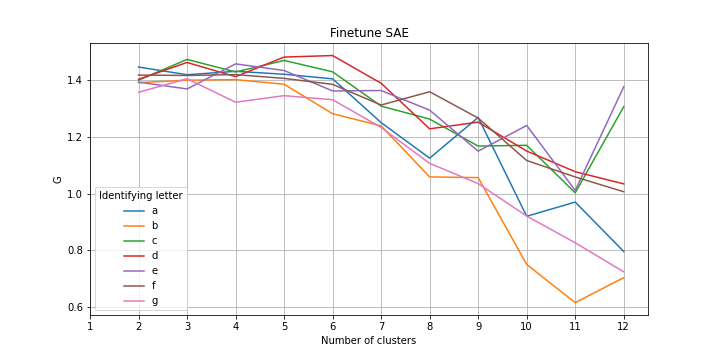
\includegraphics[width=\textwidth, keepaspectratio]{./images/Finetune_SAE_G_metric.png}
	\end{column}
	\begin{column}{0.6\textwidth}
	Clustering Model
	\centering
	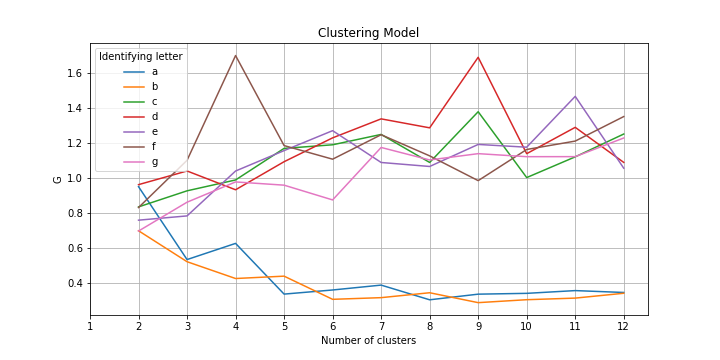
\includegraphics[width=\textwidth, keepaspectratio]{./images/Clustering_Model_G_metric.png}
	\end{column}
\end{columns}
\end{minipage}
\end{frame}

\begin{frame}{Other Clustering Model metrics}
	Cycle Accuracy
	\centering
	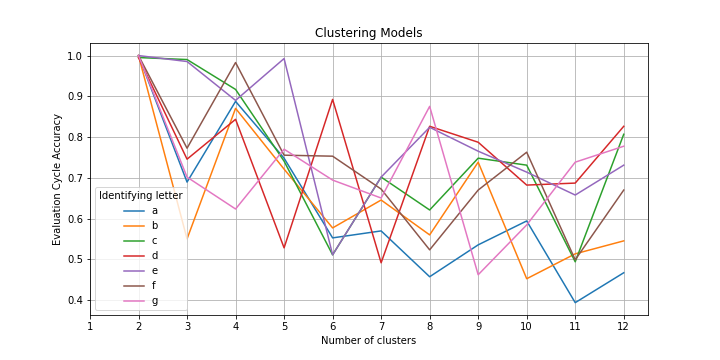
\includegraphics[width=\textwidth, keepaspectratio]{./images/clustering_cycle_acc_metric.png}
\end{frame}

\begin{frame}{Federated G metric}
\begin{minipage}[\textheight]{\textwidth}
\begin{columns}[T]
	\begin{column}{0.6\textwidth}
	SAE
	\centering
	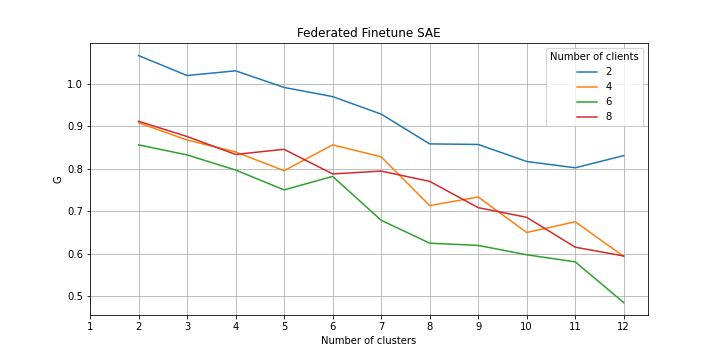
\includegraphics[width=\textwidth, keepaspectratio]{./images/fed_Finetune_SAE_G_metric.png}
	\end{column}
	\begin{column}{0.6\textwidth}
	Clustering Model
	\centering
	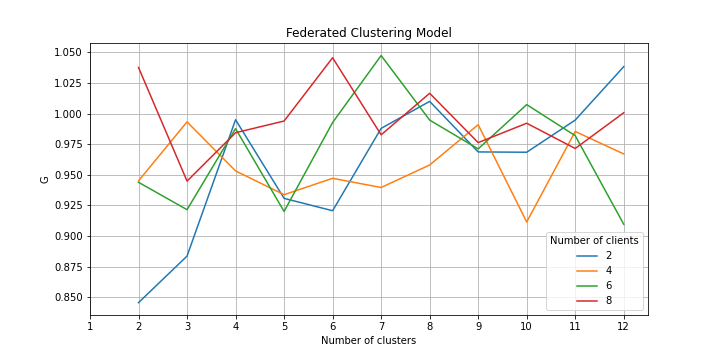
\includegraphics[width=\textwidth, keepaspectratio]{./images/fed_Clustering_Model_G_metric.png}
	\end{column}
\end{columns}
\end{minipage}
\end{frame}

\begin{frame}{Other Federated Clustering Model metrics}
	Cycle Accuracy
	\centering
	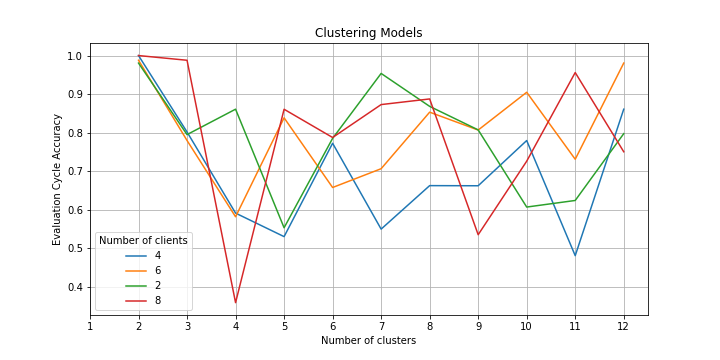
\includegraphics[width=\textwidth, keepaspectratio]{./images/fed_clustering_cycle_acc_metric.png}
\end{frame}

\section{Results}

\begin{frame}{Objective Metrics for Comparison w.r.t. HDP}
\begin{minipage}[\textheight]{\textwidth}
\begin{columns}[T]
	\begin{column}{0.6\textwidth}
	Silhouette Score 
	\centering
	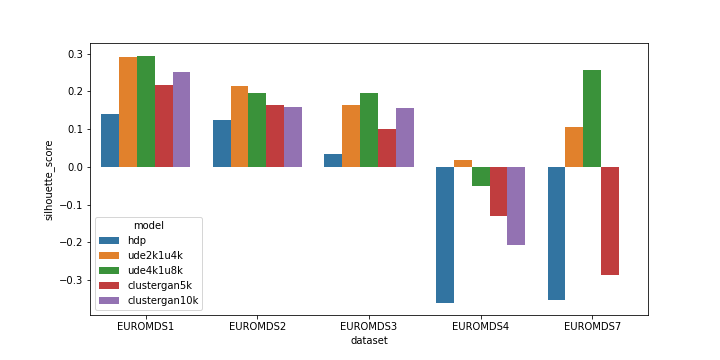
\includegraphics[width=\textwidth, keepaspectratio]{./images/silh_score.png}
	\end{column}
	\begin{column}{0.6\textwidth}
	Metrics for comparison vs HDP
	\centering
	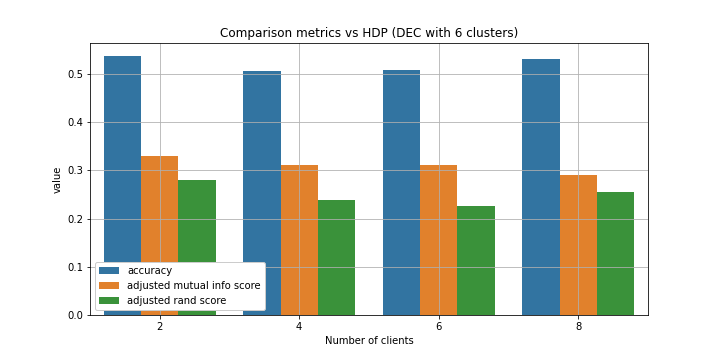
\includegraphics[width=\textwidth, keepaspectratio]{./images/metrics6.png}
	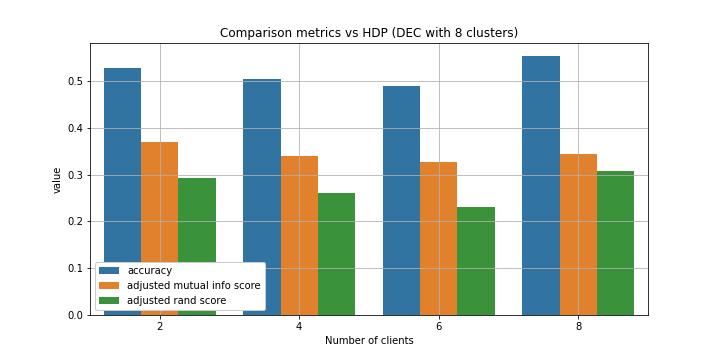
\includegraphics[width=\textwidth, keepaspectratio]{./images/metrics8.png}
	\end{column}
\end{columns}
\end{minipage}
\end{frame}

\begin{frame}{Clusters separation}
	\centering
	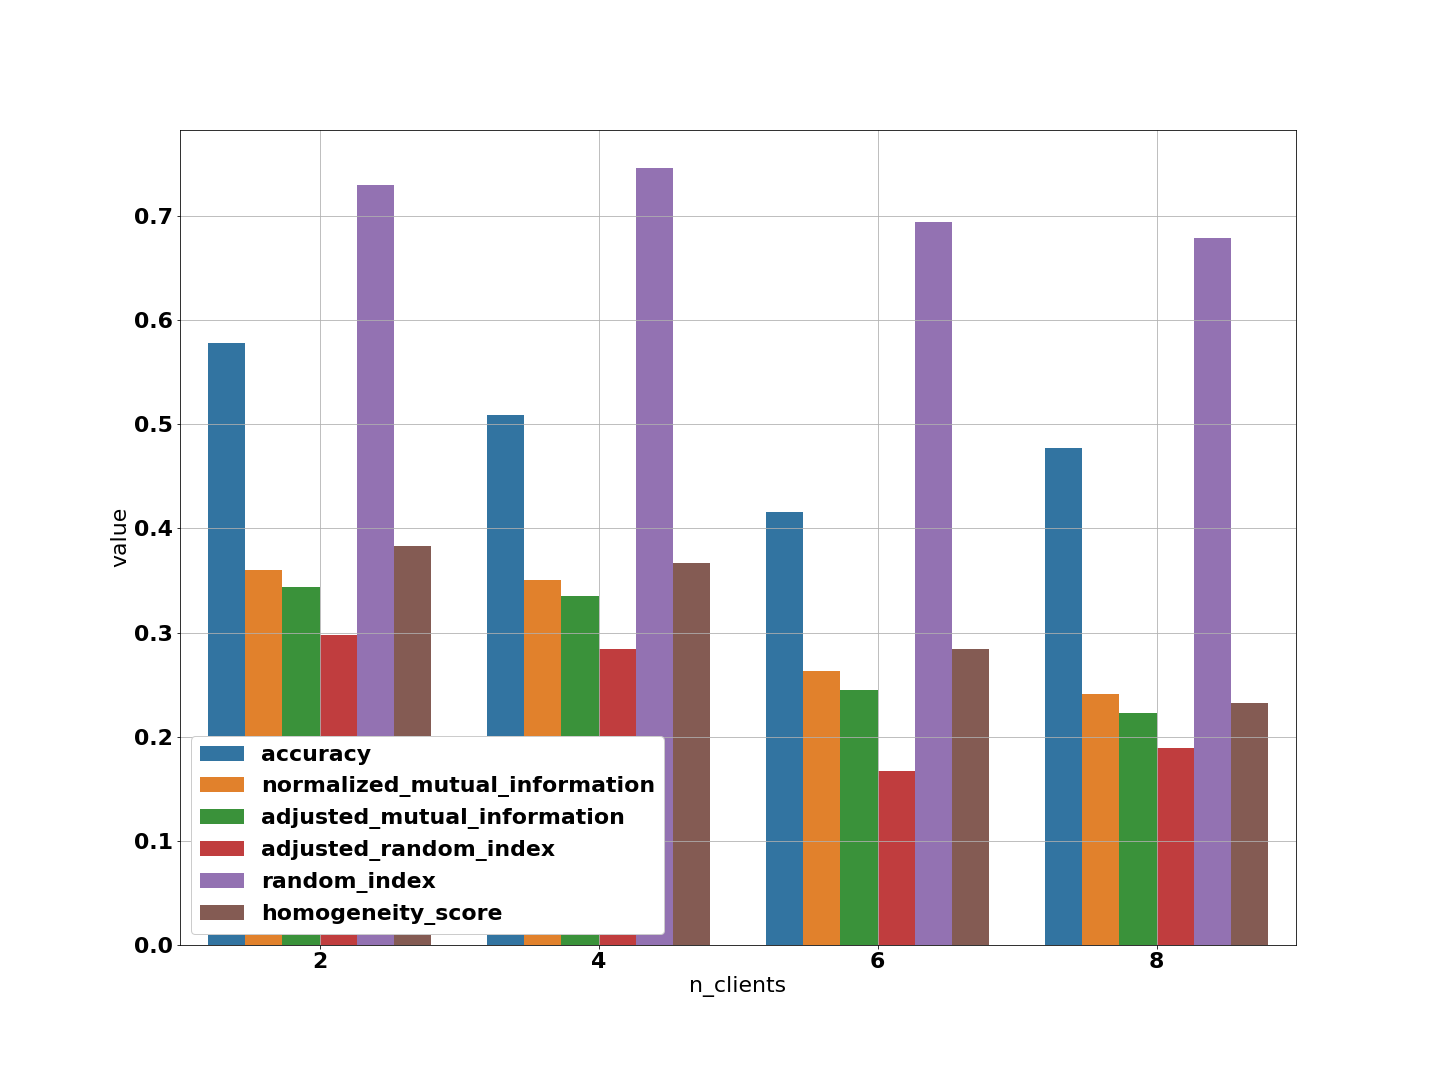
\includegraphics[width=\textwidth, keepaspectratio]{./images/metrics.png}
\end{frame}

\begin{frame}{Clusters properties}
	\centering
	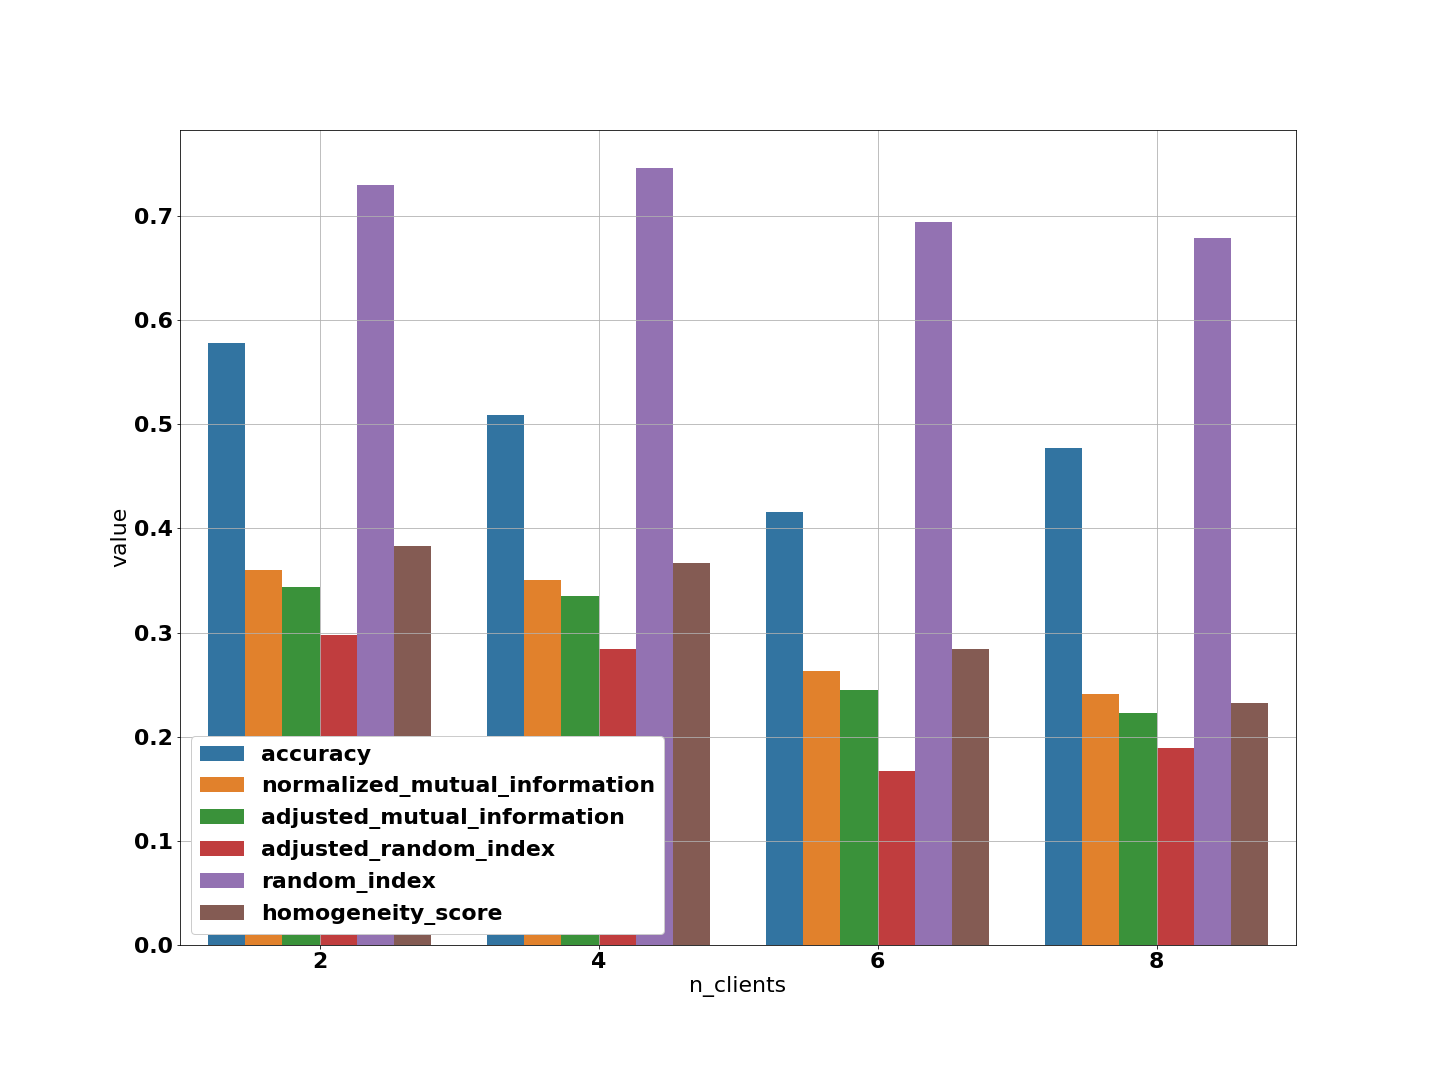
\includegraphics[width=\textwidth, keepaspectratio]{./images/metrics.png}
\end{frame}

\section{Conclusions}

\begin{frame}{Conclusions}
	\begin{itemize}
		\item Metrics and representation suggest that federated DEC separates well clusters in the feature space
		\vspace{0.5cm}
		\item Federated DEC is able to predict clusters' properties in the data space using the decoder part feeded with final centroids
	\end{itemize}
	\centering
	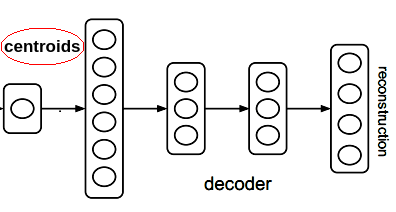
\includegraphics[width=0.7\textwidth, keepaspectratio]{./images/DEC_decoder1.png}
\end{frame}

\begin{frame}{Future work}
	\begin{itemize}
		\item Tests on different federated set-ups with different aggregation algorithms
		\vspace{0.5cm}
		\item Study proprieties of the clusters using the final DEC feature representation
		\vspace{0.5cm}
		\item Test DEC on a wider, or at least different, slice of the dataset
	\end{itemize}
\end{frame}

\section{Bibliography}

\begin{frame}{Bibliography}
	\fontsize{8pt}{7.2}\selectfont
	\bibliographystyle{plain}
	\bibliography{bibliography}
\end{frame}

\section{Final Thanks}

\begin{frame}{}
	Thanks to\\
	Gastone Castellani, Enrico Giampieri,\\Daniele Dall'Olio, Tommaso Matteuzzi\\
	\vspace{3cm}
	The End,\\
	Thanks for the attention
\end{frame}

\end{document}